\documentclass[tikz,border=2pt]{standalone}
\usetikzlibrary{calc}
\usetikzlibrary{intersections}
\usetikzlibrary{patterns}
\usepackage{bm}
\usetikzlibrary{positioning}
\usetikzlibrary{shapes}

\begin{document}

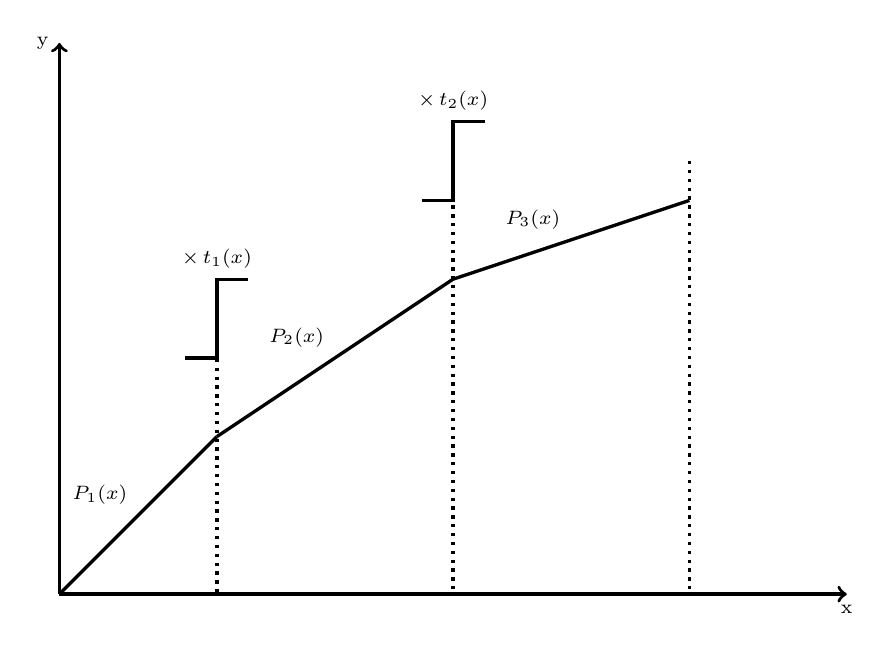
\begin{tikzpicture}[very thick]
    \tikzset{
        every node/.style={font=\scriptsize}
    }
    
    % draw axis
    \draw[->] (0,0) -- (10,0) node [below] {x};
    \draw[->] (0,0) -- (0,7) node [left] {y};

    % draw strait line 1
    \draw[solid] (0,0) -- (2,2) node[midway, above left] {$P_1(x)$};
    \draw[dotted] (2,4) -- (2,0);
    % draw strait line 2
    \draw[solid] (2,2) -- (5,4) node[midway, above left] {$P_2(x)$};
    \draw[dotted] (5,5.5) -- (5,0);
    % draw strait line 3
    \draw[solid] (5,4) -- (8,5) node[midway, above left] {$P_3(x)$};
    \draw[dotted] (8,5.5) -- (8,0);

    % \node [align=left, anchor=west] at (0,-1) {
    %     $\mbox{T2D}(x) = (1-t_1)\cdot P_1 + t_1\cdot ((1-t_2)\cdot P_2 + t_2 \cdot P_3)$ \\ \\
    %     $\mbox{T2D}(x) = (1-t_1)\cdot P_1 + t_1 \cdot (1-t_2) \cdot P_2 + t_1 \cdot t_2 \cdot P_3$
    % };

    %\node at (5,-2) {$f(x) = (1-t_1)\cdot P_1 + t_1 \cdot (1-t_2) \cdot P_2 + t_1 \cdot t_2 \cdot P_3$};

    % draw la fonction échellon / heaviside step
    \draw (1.6,3) -- (2,3) -- (2,4) -- (2.4,4); \node [above] at (2,4) {$\times \, t_1(x)$};
    \draw (4.6,5) -- (5,5) -- (5,6) -- (5.4,6); \node [above] at (5,6) {$\times \, t_2(x)$};

    % \node [align=left, anchor=west] at (0,-2.5) {
    %     $P(x) = a_{0} + a_{1}\cdot x$ \\
    %     $\displaystyle t(x) = \frac{1}{1+\exp\left(-\frac{x-x_0}{\sigma}\right)}$ , with $\sigma$ very small
    % };


\end{tikzpicture}


\end{document}